\documentclass[12pt]{article}
\usepackage{preamble}

\pagestyle{fancy}
\fancyhead[LO,LE]{Физические основы компьютерных \\ и сетевых технологий}
\fancyhead[CO,CE]{18.11.2024}
\fancyhead[RO,RE]{Лекции Музыченко Я. Б.}

\fancyfoot[L]{\scriptsize исходники найдутся тут: \\ \url{https://github.com/pelmesh619/itmo_conspects} \Cat}

\begin{document}
    \section{10. Теорема Гаусса}

    $\Phi = \oint \vec{E} d\vec{s} = \frac{q}{\varepsilon_0}$

    $d\Phi = \vec{E}d\vec{s} = E_n ds$, где $E_n = E\cos\alpha$

    \begin{minipage}{\textwidth}
        \begin{wrapfigure}{r}{0pt}
            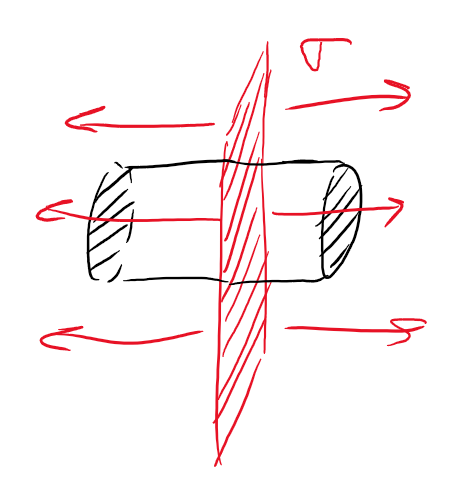
\includegraphics[width=5cm]{physics1/images/physics1_2024_11_18_1}
        \end{wrapfigure}

        \ExN{1} Однородная равномерно заряженная бесконечная плоскость, $\sigma$

        $\Phi = 2\Phi_{\text{осн}} + \cancelto{0}{\Phi_{\text{бок}}} = 2\Phi_{\text{осн}} = 2E \cdot S_{\text{осн}} = 
        \frac{a}{\varepsilon_0} = \frac{\sigma S_\text{осн}}{\varepsilon_0}$

        $E = \frac{\sigma}{2\varepsilon_0}$

        Если плоскости противоположно заряжены и расположены друг против друга, то получаем конденсатор. 
        Если плоскости имеют одноименный заряд, то между ними напряженность равна нулю
    \end{minipage}

    \begin{center}
        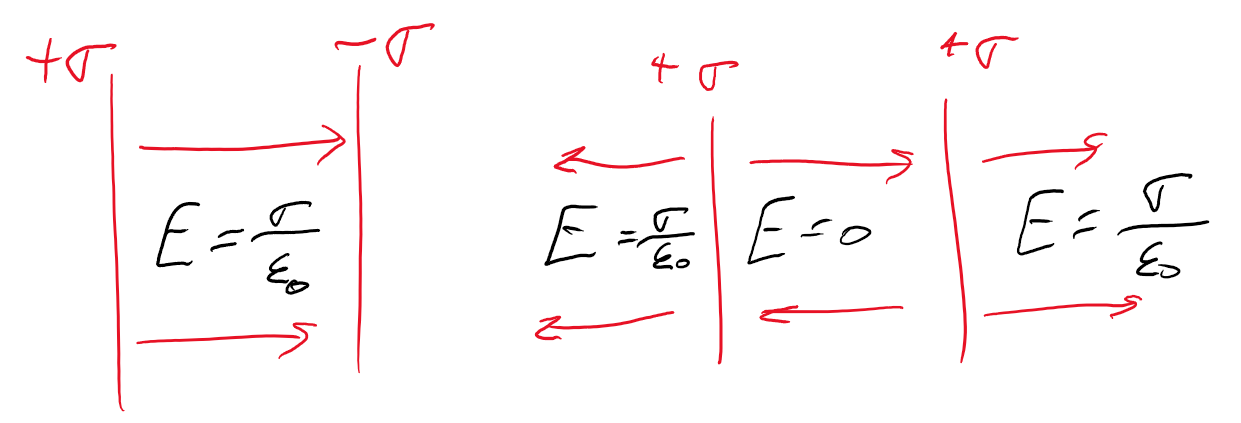
\includegraphics[width=0.8\textwidth]{physics1/images/physics1_2024_11_18_2}
    \end{center}

    \begin{minipage}{\textwidth}
        \begin{wrapfigure}{r}{0pt}
            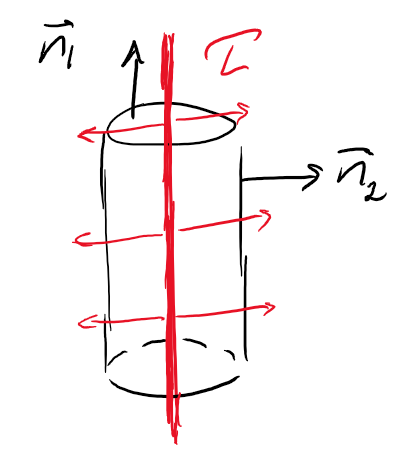
\includegraphics[width=5cm]{physics1/images/physics1_2024_11_18_3}
        \end{wrapfigure}

        \ExN{2} Цилиндрическая нить/стержень с плотностью заряда $\tau$

        Сделаем цилиндрическую поверхность вдоль стержня

        $\oint \vec{E} d\vec{s} = \frac{q}{\varepsilon_0}$

        $\oint E dS_{\text{бок}} = \frac{q}{\varepsilon_0}$

        $\vec{n}_2 \uparrow\uparrow \vec{E}$ 

        Так как $E = \mathrm{const}$ на расстоянии $r$, $E = \frac{q}{2\pi r h \varepsilon_0} = \frac{h\tau}{2\pi r h \varepsilon_0} = \frac{\tau}{2\pi r \varepsilon_0}$
    \end{minipage}


    \begin{minipage}{\textwidth}
        \begin{wrapfigure}{r}{0pt}
            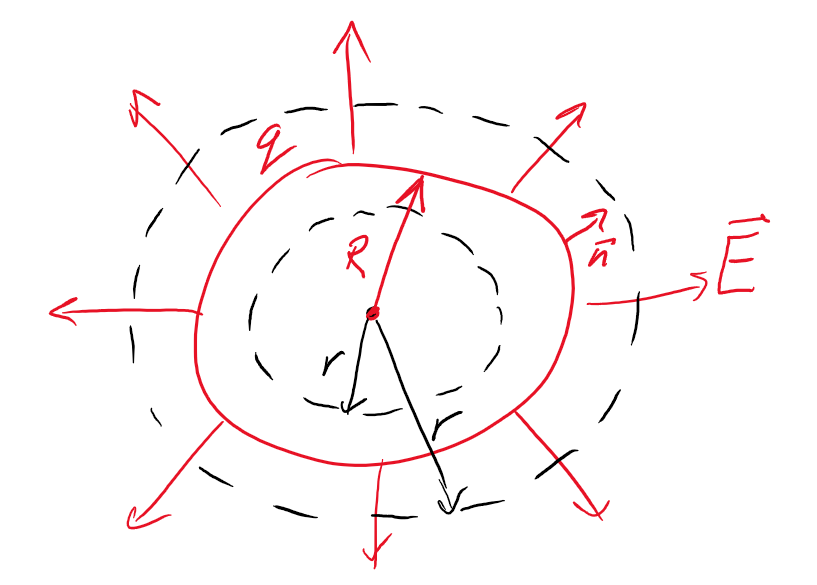
\includegraphics[width=6cm]{physics1/images/physics1_2024_11_18_4}
        \end{wrapfigure}

        \ExN{3} Сфера (пустотелая)

        Выбираем сферу радиуса $r < R$, для нее $\oint \vec{E} d\vec{s} = \frac{q}{\varepsilon_0} = 0$

        $\vec{E} = 0$ внутри сферы, так как внутри заряда нет

        Выберем сферу радиуса $r > R$

        $\oint \vec{E} d\vec{s} = \frac{q}{\varepsilon_0}$

        $E \cdot S = \frac{q}{\varepsilon_0} \qquad E = \frac{q}{4\pi \varepsilon_0 r^2}$    
    \end{minipage}

    \ExN{4} Шар (полнотелый)

    При $r \geq R$ получаем аналогичную сфере ситуацию: $E = \frac{q}{4\pi \varepsilon_0 r_2}$

    При $r < R$ $E \cdot S = \frac{q^\prime}{\varepsilon_0}$ ($q^\prime$ - заряд внутри поверхности)

    $\rho = \frac{q}{V} = \frac{q^\prime}{V^\prime} \Longrightarrow q^\prime = \frac{q \cdot r^3}{R^3}$

    $E = \frac{q \cdot r^3}{R^3} \cdot \frac{1}{4\pi r^2 \cdot \varepsilon_0} = \frac{q r}{4\pi \varepsilon_0 R^3}$

    \mediumvspace

    Так как $\vec{E}$ - поле векторное, то к нему можно применить набла-оператор. Тогда получаем:

    $\vec{\nabla} \cdot \vec{E} = \mathrm{div}\vec{E}$ - дивергенция поля

    $\vec\nabla \times \vec{E} = \mathrm{rot}\vec{E}$ - ротор поля

    По теореме Гаусса:

    $\oint \vec{E} d\vec{s} = \frac{q}{\varepsilon_0} = \frac{1}{\varepsilon_0} \int \rho dV = 
    \frac{1}{\varepsilon_0} \Pair{\rho} V$

    При $V \to 0$

    $\frac{1}{V} \oint \vec{E} d\vec{s} = \frac{1}{\varepsilon_0} \Pair{\rho}$

    $\lim_{V \to 0} \frac{1}{V} \oint \vec{E} d\vec{s} = \frac{1}{\varepsilon_0} \rho = \mathrm{div}\vec{E}$ - дивергенция поля

    Если в точке $A$ $\mathrm{div} \vec{E} < 0$, то в точке $A$ \textit{сток} поля. Если $\mathrm{div} \vec{E} > 0$, 
    то говорят, что в точке \textit{исток} поля
\end{document}

